\chapter{Caratterizzazione del Workload}
Il \var{workload} del sistema può essere visto come un insieme di tutti gli input che questo riceve durante un dato periodo di tempo. Un \var{modello di workload} è pertanto una rappresentazione che imita il comportamento del carico reale e risulta utile in quanto permette di modificare in modo semplice i parametri per osservare la risposta del sistema. Il carico di un sistema Web può essere caratterizzato a diversi livelli di astrazione. Il livello più elevato è detto di \var{business}, e si rivela utile per descrivere il carico in termini di peculiarità delle applicazioni principali; immediatamente sotto vi è il livello di \var{caratterizzazione funzionale}, il quale descrive i programmi, le richieste o le applicazioni che compongono il carico. L'ultimo livello di dettaglio, detto \var{orientato alle risorse}, consente di caratterizzare il consumo delle risorse del sistema dovuto al workload e poichè i due livelli più alti non consentono di catturare queste informazioni in modo quantitativo, si è adottato proprio quest'ultimo livello di dettaglio, in quanto è stato modellato il consumo delle risorse in termini di domanda di servizio e di intensità di carico (misurata in richieste HTTP/sec sottoposte al web server). 
\begin{figure}[H]
\begin{center}
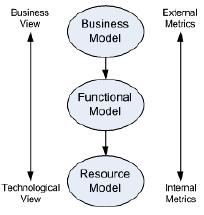
\includegraphics[scale=1.2]{etc/schema3.png}
\caption{Schema}
\label{schema3}
\end{center}
\end{figure}
Questa metrica è ben diversa dal numero di utenti che accedono in media al sistema ogni secondo, o al numero di richieste di pagine HTML sottoposte in media al sistema; in quest'ultimo caso, infatti, non si terrebbe conto dei numerosi oggetti inclusi in una pagina HTML. 
Non essendo in possesso di un carico reale (ad esempio un log di sistema), non è stato possibile effettuare un'analisi del fattore di \var{burstiness} poichè non si conoscevano il numero medio di richieste HTTP ricevute dal sistema in un determinato intervallo di tempo, nè tanto meno effettuare un'analisi analitica. Di conseguenza, la prima operazione eseguita è stata quella di effettuare un partizionamento dei documenti sulla base dei valori presentati in tabella (tabella requisiti del progetto). 
\section{Partizionamento del Carico}
I carichi reali possono presentare componenti molto eterogenee tra loro, in particolar modo per quel 
che riguarda la loro utilizzazione delle risorse del sistema; spesso la rappresentazione di un carico 
mediante una sola classe manca di accuratezza in questo senso, poiché un solo valore medio non è 
molto significativo in caso di elevata varianza dei campioni considerati. 
La motivazione per cui è utile partizionare il carico è duplice: in primo luogo la rappresentatività 
del modello di carico è incrementata, ed inoltre è molto più elevato anche il potere predittivo del 
modello stesso. Le tecniche di partizione suddividono il carico in una serie di classi le cui 
popolazioni sono omogenee secondo un qualche criterio. Il più significativo nell ambito della 
valutazione delle prestazioni è senza dubbio quello dell utilizzazione delle risorse di sistema 
A questo punto è necessario partizionare le insieme delle richieste in classi di similarità. I cosiddetti 
algoritmi di clustering sono delle tecniche che consentono di trovare dei raggruppamenti, detti 
appunto cluster, nell insieme degli elementi considerati. Questi si basano sull'individuazione di 
alcuni centroidi, ovvero elementi medi dei cluster, e cercano di assegnare ciascun elemento al 
cluster più oppurtuno mediante il calcolo della minima distanza da uno dei centroide fissati. 
Per l'analisi del caso di studio si è deciso di utilizzare il k-means che rientra nella classe degli algoritmi di clustering non-gerarchici . 
\begin{figure}[H]
\begin{center}
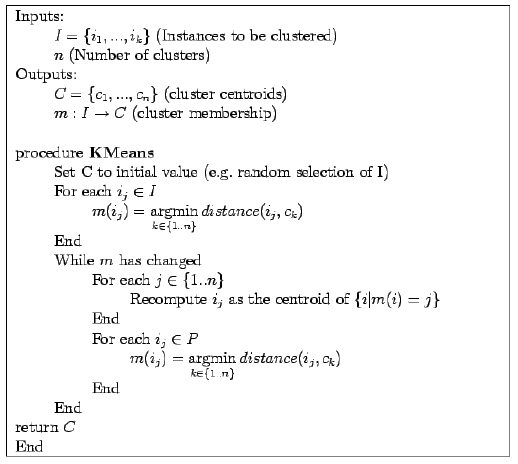
\includegraphics[scale=0.71]{etc/kmeans.png}
\caption{Schema}
\label{schema3}
\end{center}
\end{figure}
L'algoritmo K-Means è stato applicato a 10000000 documenti, generati tenendo conto delle varie distribuzioni e suddividendoli in tre classi. Si è deciso di scegliere i centroidi iniziali il più lontano possibile tra loro, prendendo come punti di riferimento i valori minimo, massimo e medio delle dimensioni dei file. I centroidi iniziali sono stati:
\begin{itemize}
\item centroide min $1.453304$
\item centroide max $715827882.666667 $
\item centroide medio $357913940.606681 $
\end{itemize}
Si è scelto di far convergere l'algoritmo nel caso in cui la differenza di valori dei centroidi tra due iterazioni successive fosse minore di $10^{-10}$ ed i risultati sono stati i seguenti: 
\begin{table}[htbp]
\begin{center}
\begin{tabular}{||c|c|c||}
\hline
Classe	&Dimensione(byte)		&Richieste \\ 
\hline\hline
1 &10281 &9999995\\ \hline
2 &279513744 &4 \\ \hline
3 &715827882 &1 \\ \hline
\end{tabular}
\end{center}
\caption{Risultati clustering}
\label{risclustering}
\end{table}
Si può notare come i documenti seguano una distribuzione \var{heavy-tailed}, dove per heavy tailed si intende dire che vi è un' elevatissima presenza di documenti di piccole dimensioni e una piccola, ma non trascurabile, presenza di documenti di dimensioni maggiori anche di diversi ordini di grandezza. Questo fenomeno è catturato dall'espressione, detta \var{Power-Law}, qui riportata 
$$P[X > x] = kx^{-\alpha}L(X)$$
in cui L(x) è una funzione che varia molto lentamente. 
Un caso particolare di questa, è la distribuzione di \var{Pareto} in cui la coda della distribuzione è esprimibile con la relazione :
$$P[X > x] = kx^{-\alpha}$$
Proprio per questa caratteristica una singola classe non può approssimare con sufficiente precisione il carico Web, dal momento che la grande variabilità degli elementi riduce il significato statistico delle misurazioni effettuate sui valori medi. 
Per ogni classe sono state inoltre ricavate le probabilità di arrivo di richieste HTTP, che torneranno utili nel momento in cui si utilizzerà il modello analitico: 
\begin{table}[H]
\begin{center}
\begin{tabular}{||c|c||}
\hline
Classe		&Prob. arrivo richieste classe R	\\
\hline
\hline
1		&0.9999995	\\
\hline
2		&0.0000004\\
\hline
3		&0.0000001\\
\hline
\end{tabular}
\end{center}
\caption{specifiche2}
\label{test_2}
\end{table}
